% DOC SETTINGS ===================================
\documentclass{article}
\usepackage[utf8]{inputenc}
\usepackage{steinmetz}
\usepackage{mathtools}  
\usepackage{multicol}
\usepackage{circuitikz}
\usepackage{listings}
\usepackage{geometry}
\usepackage{fancyhdr}
\pagestyle{fancy}
\lhead{ECE2564 Homework 3}
\rhead{Kavin Thirukonda 2021}
\fancyheadoffset{0mm}
 \geometry{
 a4paper,
 total={170mm,257mm},
 left=20mm,
 top=25mm,
 }
\mathtoolsset{showonlyrefs} 
\cfoot{}
% DOC SETTINGS ===================================
\begin{document}
\begin{center}
    “I have neither given nor received unauthorized assistance on this assignment.”
    
    
\includegraphics[width = .1\textwidth]{Signature.jpg}
\end{center}
\section*{Problem 0}
\begin{center}
    Github ID: kavnthir\\
    Github ID Number: 63033113
\end{center} 
\section*{Problem 1}
\subsection*{a)}
\begin{center}
    \boxed{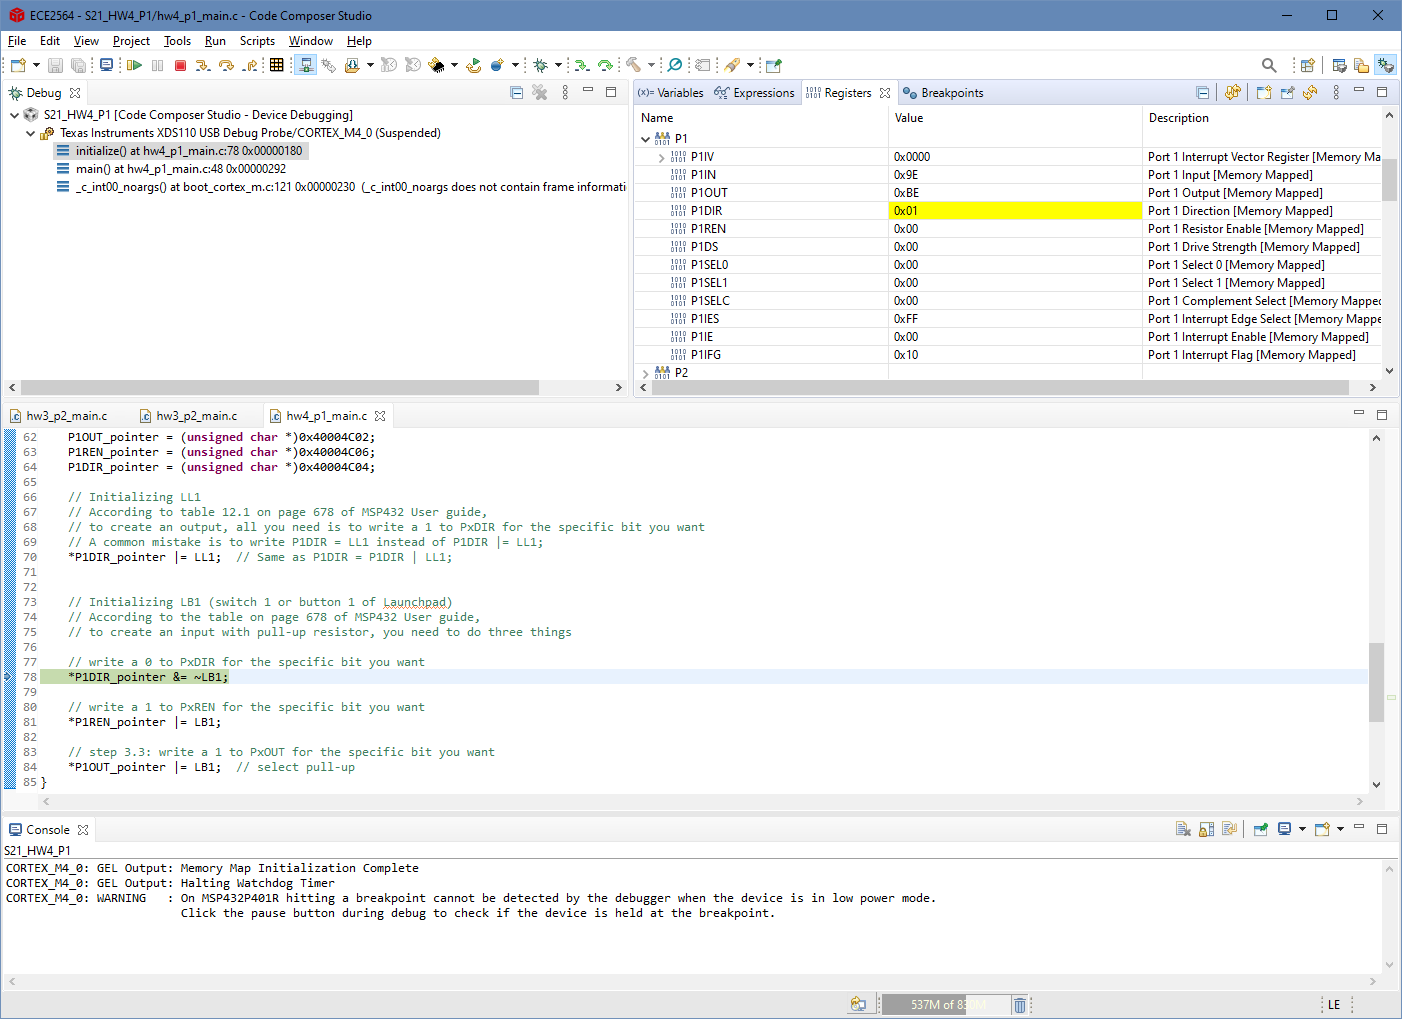
\includegraphics[width = \textwidth]{1a.png}}
\end{center}
\newpage
\subsection*{b)}
\begin{center}
    \boxed{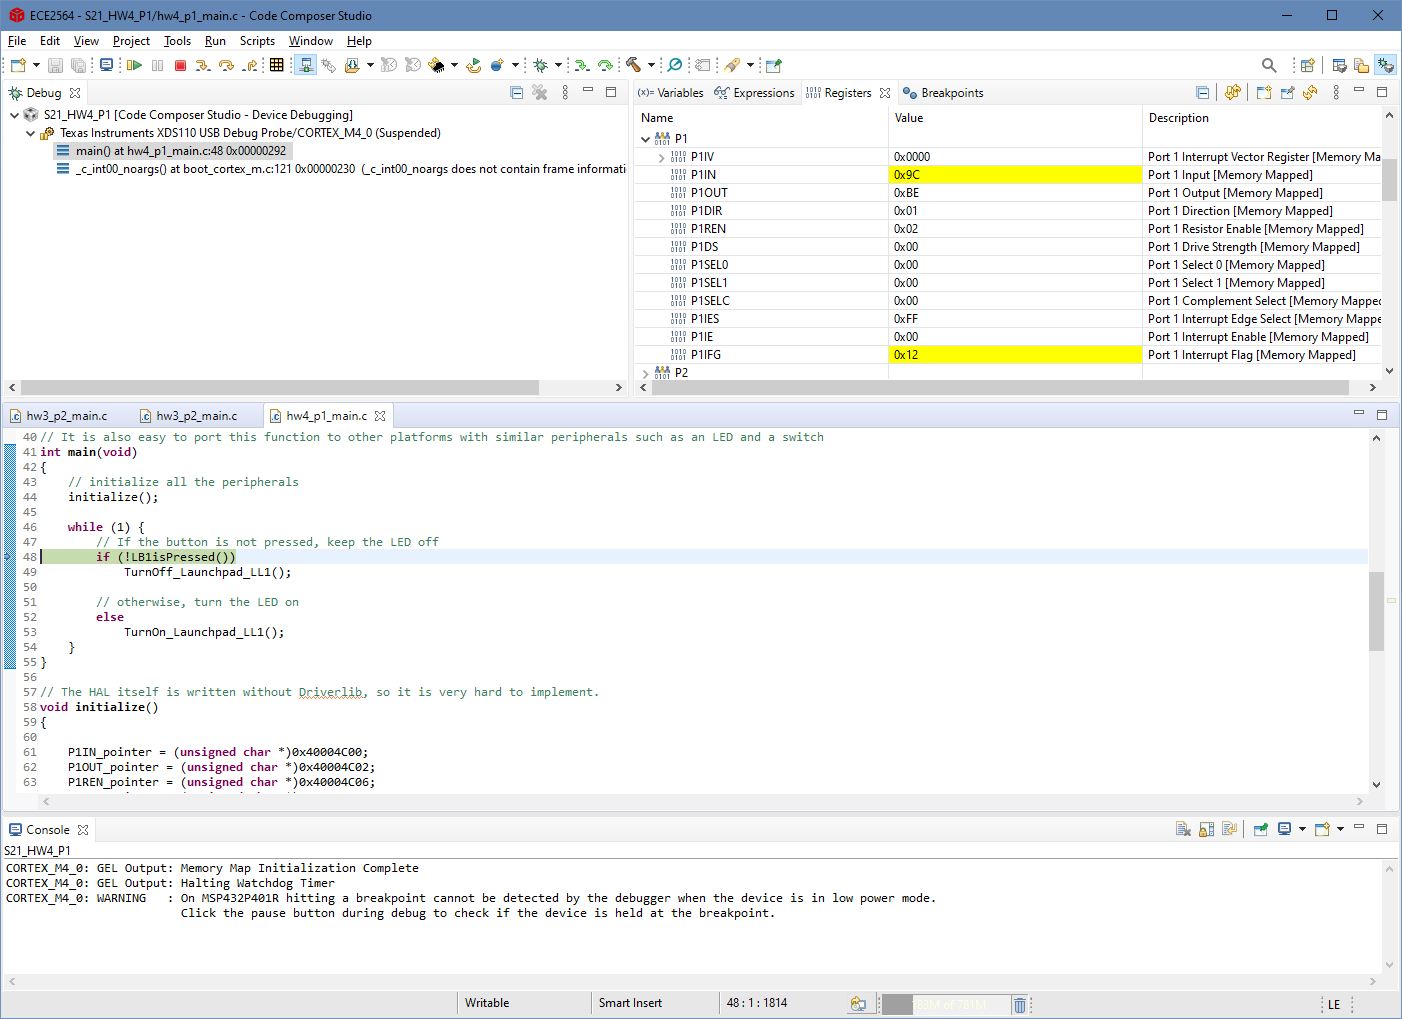
\includegraphics[width = \textwidth]{1b.png}}
    \bigbreak
    P1IN Before(Hex):0x9E\\
    P1IN After(Hex):0x9C\\
    P1IN Before(Binary):0b10011110\\
    P1IN After(Binary):0b10011100
\end{center}
\begin{center}
    When the button is pressed it goes from 0x9E to 0x9C which means that only one bit has changed between the two values, this bit on the P1IN register is named P1.1 according to the TI convention and is accordingly bit 1 of the register. Because the value is initially 1 that means that the buttons is active-low. Below is a partial diagram showing the other pins that are accounted for in the P1IN register:
    \bigbreak
    \boxed{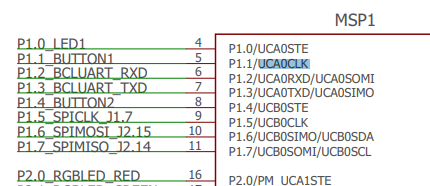
\includegraphics[width = .5\textwidth]{1b2.png}}
\end{center}
\newpage
\subsection*{c)}
\begin{center}
    P1OUT Before(Hex):0xBE\\
    P1OUT After(Hex):0xBF\\
    P1OUT Before(Binary):0b10011110\\
    P1OUT After(Binary):0b10111111
    \bigbreak
    \boxed{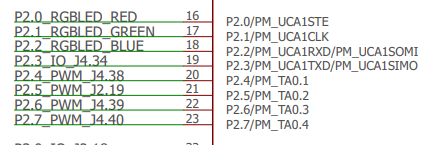
\includegraphics[width = .5\textwidth]{1c.png}}
    \bigbreak
    As we can see from the image above the bit 0 of the P2 register is the red channel of the LED, since P1OUT went high which resulted in the led turning red, this makes sense.
\end{center}
\newpage
\subsection*{d)}
\begin{center}
    \boxed{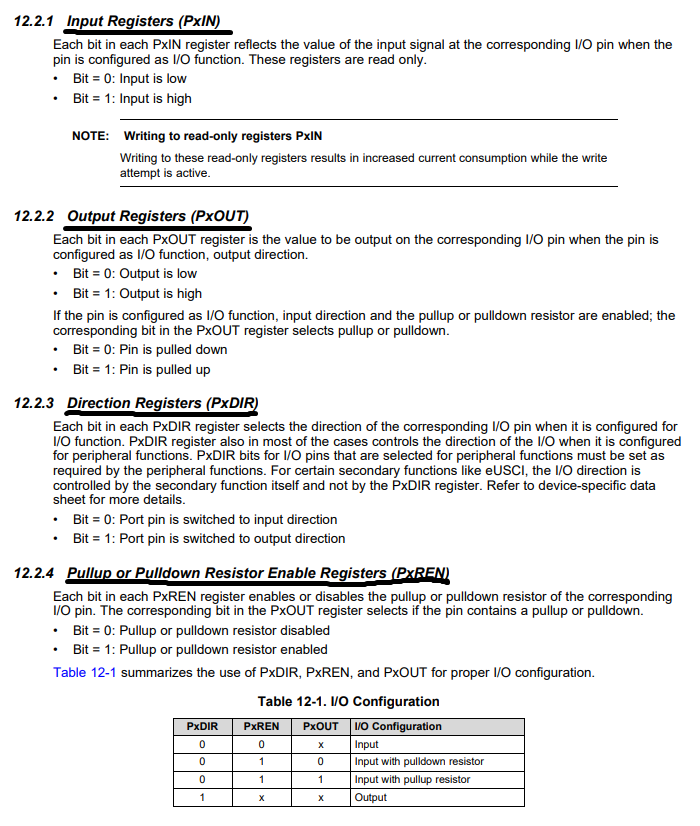
\includegraphics[width = .75\textwidth]{1d.png}}
    \boxed{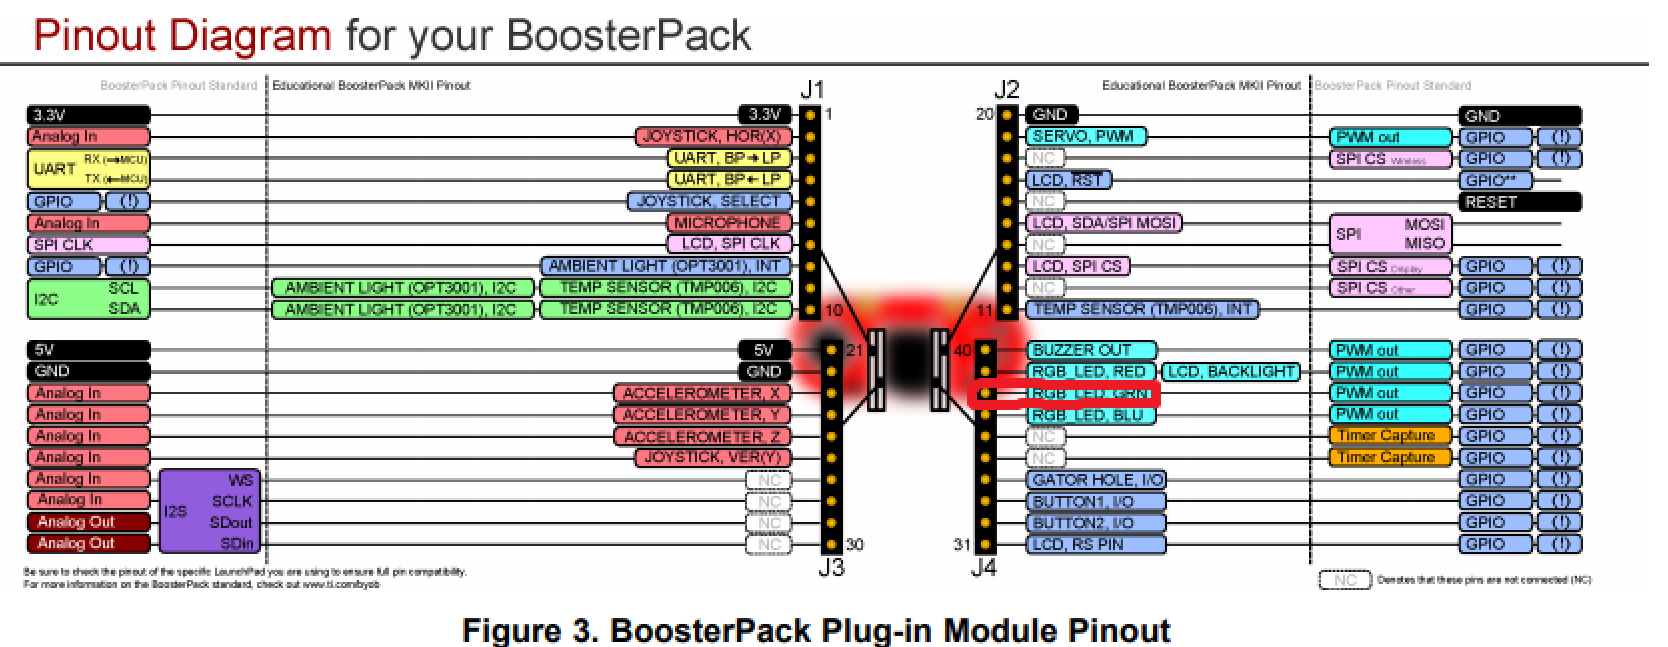
\includegraphics[width = .75\textwidth]{1d2.png}}
    \boxed{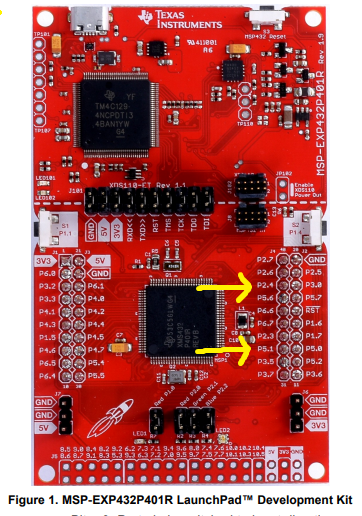
\includegraphics[width = .3\textwidth]{1d3.png}}
    \boxed{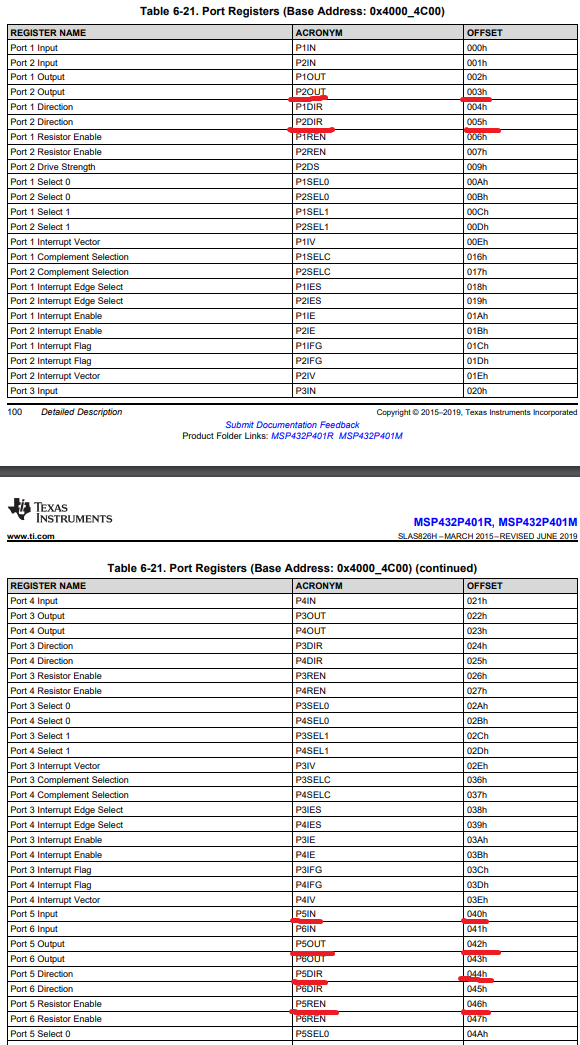
\includegraphics[width = .5\textwidth]{1d4.png}}
    \bigbreak
    Using the information found in the pictures above found in various data sheets for the two different boards I could properly piece together the code needed to make the green light be on when the button was not pushed and off when it was pushed. code for this was commited to github
\end{center}
\section*{Problem 2}
\begin{center}
    Code committed to github
\end{center}
\end{document}
